\chapter{Πρακτικό Μέρος}

\section{\en{Εργαλεία που χρησιμοποιήθηκαν}}
\en{
Η υλοποίηση αυτής της διπλωματικής έγινε χρησιμοποιώντας την γλώσσα προγραμματισμού Python. Παράλληλα, χρησιμοποιήθηκε ένα πολύ ισχυρό εργαλείο για ανάπτυξη κώδικα που ονομάζεται Jupyter Notebook.

Η Python είναι μία από τις πιο δημοφιλείς γλώσσες προγραμματισμού για τον χειρισμό δεδομένων και τον αναλυτικό προγραμματισμό (data analytics). Υπάρχουν διάφοροι λόγοι για αυτό, μερικοί εκ των οποίων είναι:
\begin{itemize}
    \item Είναι εύκολη στην εκμάθηση: Η Python είναι μια ανθρώπινη γλώσσα προγραμματισμού, η οποία σημαίνει ότι είναι σχετικά εύκολο για τους ανθρώπους να την κατανοήσουν. Αυτό την καθιστά ιδανική για χρήση σε επιστημονικά εργαστήρια όπου οι ερευνητές δεν είναι απαραίτητα ειδικοί στον προγραμματισμό.
    \itemΔιαθέτει εκτεταμένη βιβλιοθήκη: Η Python διαθέτει μια εκτεταμένη βιβλιοθήκη που περιλαμβάνει πολλά εργαλεία για τον χειρισμό των δεδομένων. Αυτό σημαίνει ότι οι ερευνητές μπορούν να χρησιμοποιήσουν ένα ευρύ φάσμα εργαλείων και λειτουργιών για την ανάλυση των δεδομένων τους. Αυτά τα πακέτα και βιβλιοθήκες περιλαμβάνουν το NumPy για επιστημονικούς υπολογισμούς, το Pandas για ανάλυση δεδομένων και επεξεργασία, το Matplotlib για οπτικοποίηση δεδομένων, και πολλά άλλα.
    \item H Python είναι μια γλώσσα ανοιχτού κώδικα, η οποία σημαίνει ότι ο κώδικας είναι διαθέσιμος για όλους να τον χρησιμοποιήσουν και να τον βελτιώσουν. Αυτό έχει ως αποτέλεσμα τη δημιουργία μιας πολύ ενεργής και ανοικτής κοινότητας που συνεργάζεται για να δημιουργήσει και να βελτιώσει τις βιβλιοθήκες και τα πακέτα που χρησιμοποιούνται στην ανάλυση δεδομένων.
\end{itemize}


Το Jupyter Notebook είναι μια διαδραστική πλατφόρμα ανάπτυξης λογισμικού, που χρησιμοποιείται για την εκτέλεση κώδικα σε πολλές γλώσσες προγραμματισμού, όπως η Python, η R, η Julia και άλλες. Επιτρέπει στους χρήστες να δημιουργούν και να κοινοποιούν ένα αρχείο σε μορφή notebook που περιέχει κώδικα, αποτελέσματα, εξηγήσεις, εικόνες, γραφήματα και πίνακες.

Τα notebooks αποτελούνται από σελίδες, οι οποίες μπορούν να περιέχουν κελιά κώδικα και κελιά κειμένου. Τα κελιά κώδικα περιέχουν τον κώδικα που εκτελείται σε πραγματικό χρόνο και παράγει τα αποτελέσματα, ενώ τα κελιά κειμένου χρησιμοποιούνται για να παρέχουν εξηγήσεις, οδηγίες ή σχόλια σχετικά με τον κώδικα. Το Jupyter Notebook επιτρέπει στους χρήστες να επεξεργάζονται τα κελιά κώδικα και κειμένου σε πραγματικό χρόνο, επιτρέποντας την αμφίδρομη επικοινωνία με τον κώδικα και τα αποτελέσματα που παράγει.
}


\section{Το \en{dataset}}
Στο κεφάλαιο αυτό αρχικά γίνεται μια περιγραφή το συνόλου δεδομένων \en{(dataset)}  που χρησιμοποιήθηκε για την εκπόνηση της παρούσας εργασίας. 

\subsubsection{Πηγή \en{dataset}}
Το θέμα του ιατρικού απορρήτου καθιστά τη συλλογή και διάθεση ιατρικών δεδομένων δύσκολη διαδικασία. Για το λόγο αυτό, είναι γνωστό στην επιστημονική κοινότητα ότι αποτελούν σπάνια και δύσκολα προσβάσιμη πληροφορία. Το συγκεκριμένο \en{dataset} αντλήθηκε από χρήστες της πλατφόρμας \en{kaggle} \cite{dataset}, με την κύρια πηγή άντλησης να είναι η ιστοσελίδα \en{www.mtsamples.com}. \cite{mtsamples}
Φυσικά, όλες οι εγγραφές είναι απολύτως ανώνυμες. Η πρόκληση του \en{kaggle} είναι η επιτυχής πρόβλεψη της ιατρικής ειδικότητας κάθε περιγραφής ιατρικού περιστατικού.

\subsubsection{Δομή \en{dataset}}
Η αρχική μορφή του \en{dataset} είναι ένα αρχείο \en{csv} με πέντε χιλιάδες (5000) εγγραφές και έξι (6) πεδία και η δομή του έχει ως εξής:
\begin{enumerate}
    \item Α/Α - (Αύξων αριθμός εγγραφής)
    \item \en{description} - (Περιγραφή)
    \item \en{medical specialty} - (Ιατρική ειδικότητα)
    \item \en{sample name} - (Όνομα δείγματος)
    \item \en{transcription} - (Ιατρική συνταγογράφηση)
    \item \en{keywords } - (Λέξεις - κλειδιά)
\end{enumerate}
\clearpage

\begin{figure} [ht!]
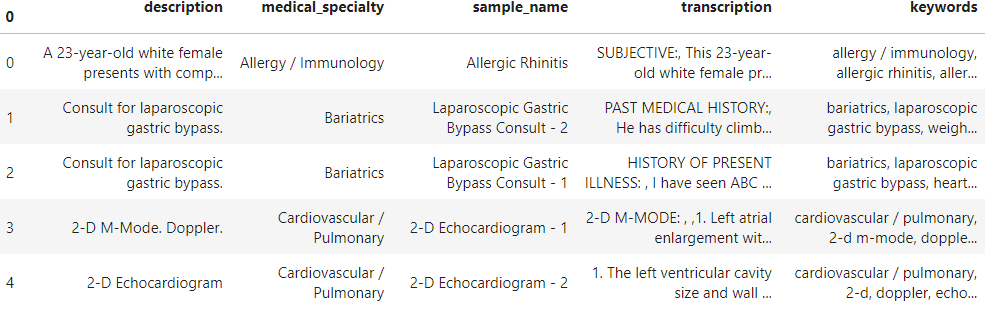
\includegraphics[width=\textwidth,height=\textheight,keepaspectratio]{pictures/3dataset5sthles.png} \caption{Οι πέντε (5) πρώτες στήλες του \en{dataset}}\label{figure3.1}
\end{figure}
Το Σχήμα~ \ref{figure3.1} απεικονίζει ενδεικτικά τις πέντε (5) πρώτες στήλες του \en{dataset} πριν υποστεί οποιαδήποτε επεξεργασία, όπως γίνεται η εισαγωγή του αρχείου \en{csv} στο πρόγραμμα.


Σε πρώτο στάδιο ανάλυσης του συνόλου δεδομένων και με χρήση κατάλληλων εντολών \en{python} εξάγονται πληροφορίες για τον αριθμό των κατηγοριών (Ιατρικών ειδικοτήτων), το όνομα κάθε κατηγορίας καθώς και το πλήθος εγγραφών που περιέχει.

\begin{figure} [ht!]
\centering
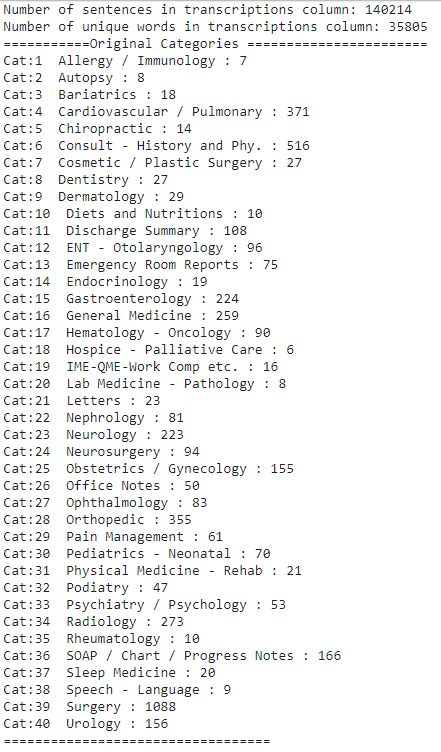
\includegraphics[width=\textwidth,height=20cm,keepaspectratio]{pictures/3categories.png} \caption{Η αρχική κατανομή των δεδομένων στις κατηγορίες}\label{figure3.2}
\end{figure}

Το Σχήμα~ \ref{figure3.2} εμφανίζει τις σαράντα (40) κατηγορίες που περιέχει αρχικά το \en{dataset} καθώς και το πλήθος εγγραφών ανά κατηγορία.

Επίσης, δημιουργείται η συνάρτηση \en{get\_sentence\_word\_count()}, η οποία μας επιστρέφει το πλήθος των διακριτών λέξεων και προτάσεων που υπάρχουν στο πεδίο \en{transcription} του εισαγόμενου αρχείου.
Έτσι έχουμε μια πιο ολοκληρωμένη εικόνα για τη μορφή, τη δομή και την κατανομή των δεδομένων στο αρχείο.

Το επόμενο στάδιο που περιγράφεται στο κεφάλαιο 3 είναι το στάδιο της Προεπεξεργασίας. Η σωστή και καθαρή απεικόνιση των δεδομένων βοηθάει τον ερευνητή να εφαρμόσει πιο στοχευμένες και αποτελεσματικές τεχνικές προεπεξεργασίας κειμένου ώστε να αποφύγει την απώλεια χρήσιμης πληροφορίας. 


\clearpage
\section{Προεπεξεργασία \en{(Preprocessing)}}
Στο κεφάλαιο αυτό  παρουσιάζεται αναλυτικά το στάδιο της Προεπεξεργασίας \en{(Preprocessing)}. Θα παρουσιαστούν εκτενώς όλες οι μέθοδοι και οι τεχνικές που χρησιμοποιήθηκαν, ο σκοπός τους και η τελική μορφή των δεδομένων. 

Είναι σημαντικό να γίνει κατανοητή η σημαντικότητα αυτού του σταδίου για την ακρίβεια των τελικών αποτελεσμάτων. Το αρχικό μας σύνολο δεδομένων περιέχει δύο είδη πληροφορίας. Τη χρήσιμη για τον ερευνητικό σκοπό και όλη την υπόλοιπη η οποία, εάν δεν απομονωθεί σωστά, ενδέχεται να προκαλέσει αλλοίωση των αποτελεσμάτων, εκπαίδευση του συστήματος προς λανθασμένη κατεύθυνση και σίγουρα ανώφελη κατανάλωση υπολογιστικής ισχύος αλλά και χρόνου.

Σε αυτό το στάδιο ο ερευνητής πρέπει να παρατηρήσει σωστά την πληροφορία και να κρατήσει το ωφέλιμο κομμάτι με σκοπό να έχει πιο ποιοτικά δεδομένα, προσέχοντας στην προσπάθεια αυτήν να μην απωλέσει κομμάτι χρήσιμης πληροφορίας που θα εκπαίδευε σωστά το σύστημα.


\subsection{Βήμα 1: Μείωση κατηγοριών και απομόνωση πεδίων}
Είδαμε οτι στο συγκεκριμένο \en{dataset} υπάρχει μεγάλη ανομοιομορφία ως προς την κατανομή των δεδομένων στις διάφορες κατηγορίες. Αυτό αποτελεί ένα μείζον πρόβλημα στους αναλυτές δεδομένων, γνωστό ως \en{Imbalanced Data}, το οποίο οδήγησε την κοινότητα στην ανάπτυξη διάφορων τεχνικών αντιμετώπισης του. Το μεγαλύτερο πρόβλημα έγκειται στο ότι οι αλγόριθμοι ταξινόμησης υποθέτουν οτι όλες οι κλάσεις έχουν ίδο πλήθος δεδομένων και εκπαιδεύονται εξ'ίσου σε όλες.

Επομένως, στο πρώτο βήμα, εξαλείφουμε τις μειονότητες με σκοπό να οδηγηθούμε σε ένα κάπως πιο ισορροπημένο σύνολο δεδομένων. Πρατικά, φιλτράρουμε τα δεδομένα έτσι ώστε να εξαλειφθούν οι κατηγορίες που έχουν λιγότερα απο 50 στοιχεία. 

Εμφανίζουμε ξανά το πλήθος των κατηγοριών και των εγγραφών ανά κατηγορία, καθώς και τη γραφική απεικόνιση σε διάγραμμα μέσω της βιβλιοθήκης \en{matplotlib}. Τα αποτελέσματα φαίνονται στα Σχήματα ~\ref{figure4.1} και ~\ref{figure4.2}
\clearpage

\begin{figure}\centering
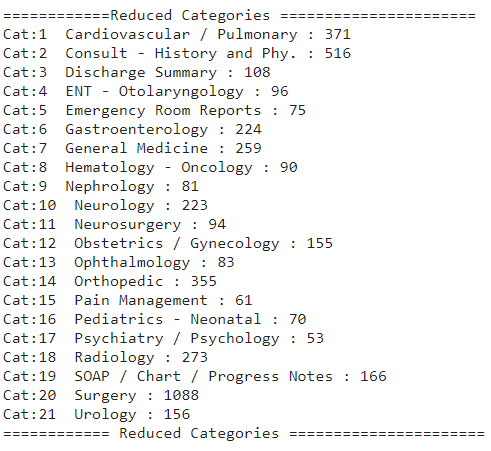
\includegraphics[width=\textwidth,height=9cm,keepaspectratio]{pictures/3reducedCategories.png} \caption{Το πλήθος εγγραφών ανά κατηγορία μετά την εξάλειψη των μειονοτήτων.}\label{figure4.1}
\end{figure}

\begin{figure}\centering
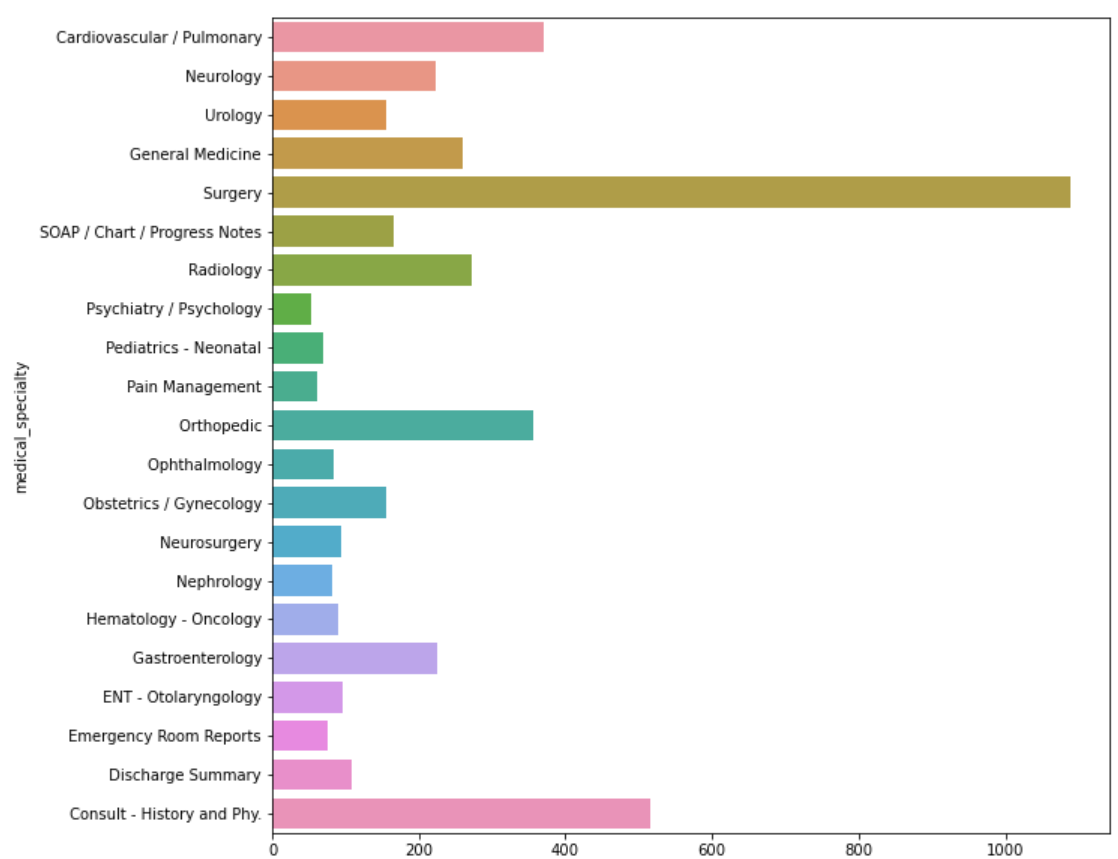
\includegraphics[width=\textwidth,height=14cm,keepaspectratio]{pictures/3categoriesPlot.png} \caption{Γραφικη απεικόνιση του σχήματος 4.1}\label{figure4.2}
\end{figure}
\clearpage
Είδαμε ότι το σύνολο των δεδομένων αποτελείται απο έξι πεδία εκ των οποίων μας αφορούν μόνο δύο:

1) Το πεδίο \en{medical\_specialty} το οποίο αναφέρεται στην κατηγορία/ειδικότητα στην οποία έγκειται το περιστατικό και 

2) Το πεδίο \en{transcription} το οποίο είναι το κυρίως κείμενο και αναφέρεται στην περιγραφή του περιστατικού.  

Επομένως τα δεδομένα φιλτράρoνται ξανά με σκοπό να κρατηθεί μόνο η πληροφορία αυτών των δύο πεδίων και στη συνέχεια αποθηκεύονται σε έναν πίνακα, εμφανίζοντας στο τέλος το πλήθος στηλών και γραμμών. 

Τα δεδομένα πλέον έχουν την εξής μορφή : \en{[4597 rows x 2 columns]}

\subsection{Βήμα 2: Kαθαρισμός κειμένου (\en{text cleaning})}

Στη συνέχεια εκτελείται η διαδικασία καθαρισμού κειμένου (\en{text cleaning process.}) Αρχικά ορίζονται δύο συναρτήσεις: η \en{clean\_text()} και η \en{lemmatize\_text()} οι οποίες επιτελούν τις παρακάτω διεργασίες: 
\begin{enumerate}
    \item Διαίρεση σε όρους \en{(Tokenization)}:
    Με αυτόν τον όρο αναφερόμαστε τον κατακερματισμό μιας συμβολοσειράς σε διακριτές λέξεις. Ο κάθε όρος μπορεί να είναι ολόκληρη λέξη, μεμονομένος χαρακτήρας, αριθμός, σύμβολο ή σημείο στίξης. \cite{lemmatize}. Σε αυτήν την εργασία, η κάθε εγγραφή του πεδίου \en{transcription}, που αποτελούν το κείμενο προς επεξεργασία, χωρίζεται σε λέξεις. Η μορφή των δεδομένων τώρα είναι ένας πίνακας όπου το κείμενο παρουσιάζεται σε μορφή λίστας με διακριτούς όρους.
    
    \item Αφαίρεση λέξεων χωρίς νοηματική αξία \en{stopwords removal}:
    Ένα από τα πιο συνηθισμένα βήματα προεπεξεργασίας κειμένου φυσικής γλώσσας είναι η αφαίρεση λέξεων χωρίς ιδιαίτερη νοηματική αξία. Η βιβλιοθήκη \en{NLTK} της \en{Python} προσφέρει αυτή τη δυνατότητα, απομακρύνοντας λέξεις που δεν αποδίδουν χρήσιμη πληροφορία, αντιθέτως προσθέτουν στο κείμενο θόρυβο και όγκο. Αυτό γίνεται είτε μέσω έτοιμης λίστας \en{stopwords}, είτε εντοπίζοντας λέξεις που εμφανίζονται εξαιρετικά συχνά σε ένα κείμενο. Τέτοιες λέξεις μπορεί να είναι άρθρα, αντωνυμίες, ακόμα και πολύ συνηθισμένα ρήματα.
    
    \item Μετατροπή κεφαλαίων χαρακτήρων σε πεζούς:
    Εδώ γίνεται χρήση της μεθόδου \en{.lower()} που προσφέρει η  \en{python} για μετατροπή συμβολοσειρών, η οποία μετατρέπει οποιοδήποτε κεφαλαίο χαρακτήρα σε πεζό.
    
    \item Απομάκρυνση αριθμών και συμβόλων:
    Οι αριθμοί, τα σύμβολα και τα σημεία στίξης, για το σκοπό της εργασίας, αποτελούν περιττή πληροφορία. Απαλάσσοντας το κείμενο από αυτά μειώνεται ο όγκος εργασίας, η απαιτούμενη υπολογιστική ισχύς και παράγονται πιο ποιοτικά δεδομένα. Έτσι με χρήση κατάλληλων εντολών της \en{python}, όλα αυτά αφαιρούνται.
    
    \item \en{Stemming}
    Ο όρος \en{Stemming} αναφέρεται σε μια διαδικασία που παρέχεται απο τη βιβλιοθήκη \en{NLTK} της \en{Python} η οποία ανάγει όλες τις ομόρριζες λέξεις του κειμένου στην αρχική τους ρίζα, αδιαφορώντας για τις διαφορετικές καταλήξεις που ενδεχομένως να έχουν. Για παράδειγμα, η λέξη \en{coding} ανάγεται στη λέξη \en{code}.
    
    \item Λημματοποίηση \en{(Lemmatization)}
    Ο όρος λημματοποίηση αναφέρεται στη διαδικασία επεξεργασίας κειμένου φυσικής γλώσσας με σκοπό να φέρει την κάθε λέξη σε μια μορφή τέτοια, ώστε να υπάρχει όσο το δυνατόν μικρότερη ποικιλία στο συνολικό λεξιλόγιο, επιδιώκοντας την επιστροφή των λέξεων στο αρχικό τους λήμμα. Η βασική διαφορά των δύο τελευταίων διαδικασιών ειναι οτι στη λημματοποίηση εξετάζεται η γλωσσολογική προέλευση κάθε όρου ώστε να βρεθεί το κατάλληλο λήμμα. Αποτελεί μια πιο εξελιγμένη διαδικασία καθώς το \en{stemming} δεν εξετάζει πληροφορίες που αφορούν τη γλωσσολογική προέλευση της λέξης, αλλά μόνο τη σχέση ρίζας - κατάληξης. Χρησιμοποιώντας και πάλι τη βιβλιοθήκη \en{NLTK} της \en{Python}, γίνεται ομαδοποίηση των λημμάτων μέσω της μεθόδου \en{WordNetLemmatizer()} με βάση το λεξικό \en{WordNet} Για παράδειγμα, στο \en{lemmatization}, η λέξη \en{better} ανάγεται στη λέξη \en{good}.
\end{enumerate}

Σε αυτό το σημείο, η λίστα κειμένων είναι απαλλαγμένη από στοιχεία που προσδίδουν αχρείαστο όγκο, θόρυβο και περιττή πληροφορία. Στα επόμενα κεφάλαια θα χρησιμοποιηθεί το σύνολο δεδομένων με το "καθαρισμένο" κείμενο ως είσοδο στα προγράμματα με σκοπό την εκπαίδευση του συστήματος και την παραγωγή γνώσης.

\clearpage
\section{Υλοποίηση Ταξινόμησης}
Στο προηγούμενο κεφάλαιο φάνηκε αναλυτικά πως τα δεδομένα του \en{dataset} έφτασαν μέσω των διαφόρων διεργασιών της προεπεξεργασίας σε μια πιο ποιοτική και καθαρή μορφή. Για να φανεί χρήσιμη η πληροφορία αυτή, χρειάζεται το αδόμητο κείμενο να μετατραπεί σε κάποια κατανοητή μορφή για τους υπολογιστές, όπως πίνακες ή διανύσματα από χαρακτηριστικά (features).

Αυτό γίνεται με χρήση της μεθόδου \en{tf-idf}, ο τρόπος λειτουργίας της οποίας αναλύθηκε σε προηγούμενο κεφάλαιο. 

Έπειτα, το Σχήμα~ \ref{figure5.1} εμφανίζει την απεικόνιση του πίνακα που προέκυψε από την \en{tf-idf} με χρήση της μεθόδου \en{t-SNE} όπου γίνεται εμφανές πως πολλές κατηγορίες-ειδικότητες αλληλοκαλύπτονται.

\begin{figure} [ht!]
\centering
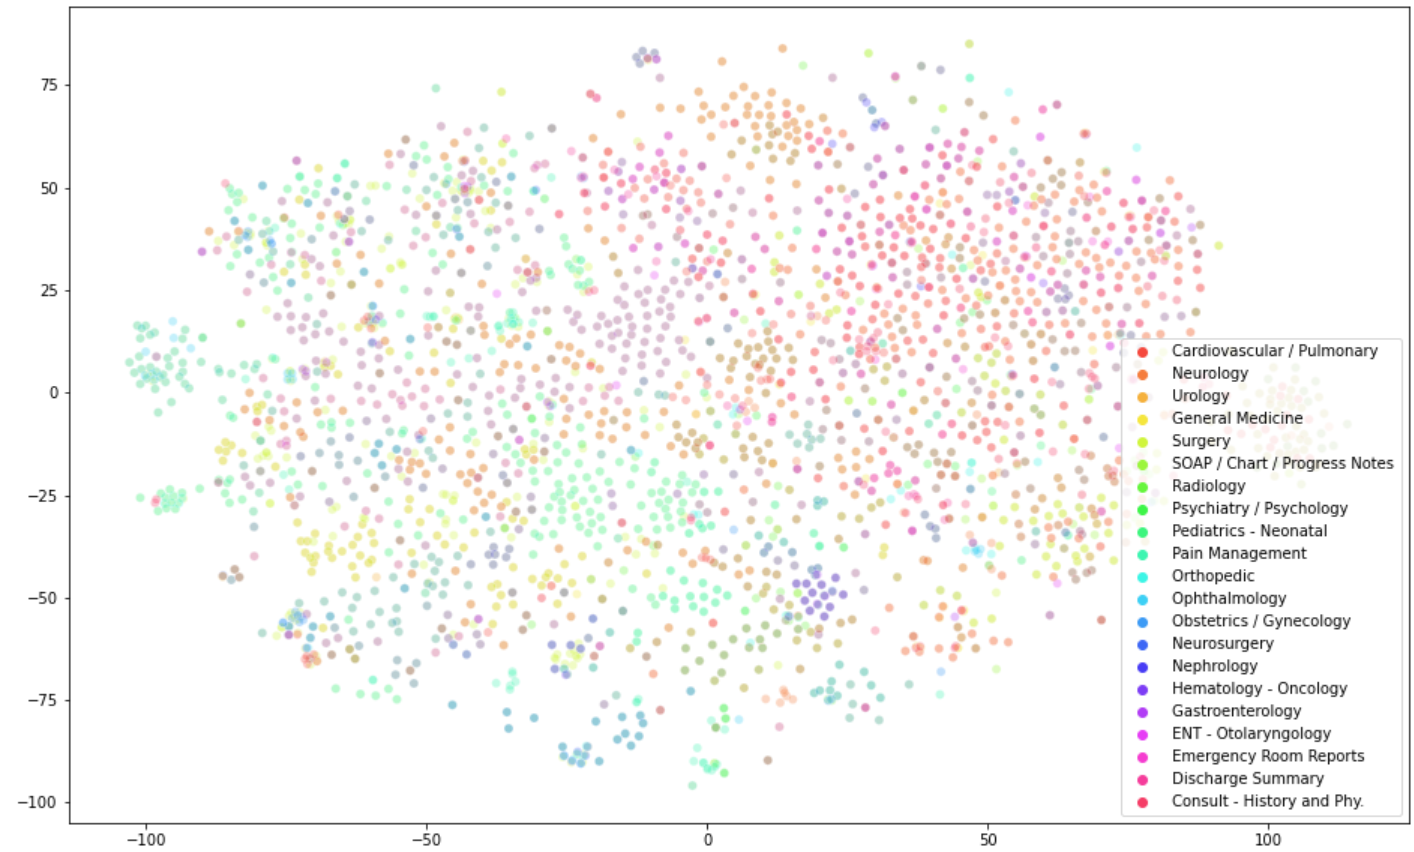
\includegraphics[width=\textwidth,height=20cm,keepaspectratio]{pictures/5.1tsne.png} 
\caption{Η γραφική απεικόνιση του αλγορίθμου \en{t-SNE}}\label{figure5.1}
\end{figure}

Στη συνέχεια εφαρμόζεται η μέθοδος \en{PCA} στον πίνακα \en{tf-idf} με στόχο τη μείωση διαστατικότητας. 

Η \en{Sklearn (ή Scikit-learn)} είναι μια βιβλιοθήκη της \en{Python} η οποία προσφέρει διάφορες δυνατότητες για επεξεργασία δεδομένων και χρησιμοποιείται συνήθως για ταξινόμηση, ομαδοποίηση και επιλογή μοντέλου. 

Για να εκπαιδεύσουμε το μοντέλο χρησιμοποιώντας ένα συγκεκριμένο \en{dataset} θα πρέπει να το «τεστάρουμε» πάνω σε ένα δεύτερο \en{dataset}. Όταν έχουμε μόνο ένα, όπως στη δική μας περίπτωση, το χωρίζουμε στα δύο χρησιμοποιώντας τη μέθοδο \en{train\_test\_split()} της \en{sklearn}. 
Η μέθοδος αυτή χωρίζει το σύνολο των \en{data arrays} σε δύο υποσύνολα: \en{training set} (Σύνολο εκπαίδευσης) και \en{test set} (Σύνολο αξιολόγησης). 

Έτσι, μετά την εφαρμογή του διαχωρισμού έχουμε:
\begin{itemize}
    \item \en{Train\_Set\_Size: (3447, 587) }
    \item \en{Test\_Set\_Size: (1150, 587) }
\end{itemize}


Στη συνέχεια, εφαρμόζουμε στα δεδομένα Λογιστική Παλινδρόμηση \en{(Logistic Regression)} για να εκπαιδεύσουμε το μοντέλο στα \en{training data} και να κάνει την πρόβλεψη στα \en{test data}.
Η εφαρμογή της λογιστικής παλινδρόμησης στη βιβλιοθήκη της \en{Python} \en{scikit-learn} μπορεί να προσεγγιστεί από την κλάση \en{LogisticRegression}. 


Μετά απο αυτήν τη διαδικασία κατασκευάζουμε τον πίνακα σύγχυσης (\en{confusion matrix}). 
Πρόκειται για έναν \en{MxM} πίνακα, όπου το \en{(i,j)} στοιχείο του ισούται με το πλήθος των σημείων που, ενώ προέρχονται από την κλάση \en{i}, καταχωρούνται στην κλάση \en{j}. 
Δίνει πληροφορίες σχετικά με το αν κάποιες κλάσεις έχουν την τάση να συγχέονται με άλλες κλάσεις.

Από τη γραφική απεικόνιση του πίνακα σύγχυσης που φαίνεται στο Σχήμα~ \ref{figure5.3}, παρατηρούμε πως μεγαλύτερη σύγχυση υπάρχει σε συγκεκριμένες ειδικότητες όπως η χειρουργική, οι οποίες έχουν την ιδιότητα υπερκλάσης, αφού επικαλύπτονται με άλλες ειδικότητες εκ φύσεως.

\begin{figure} [ht!]
\centering
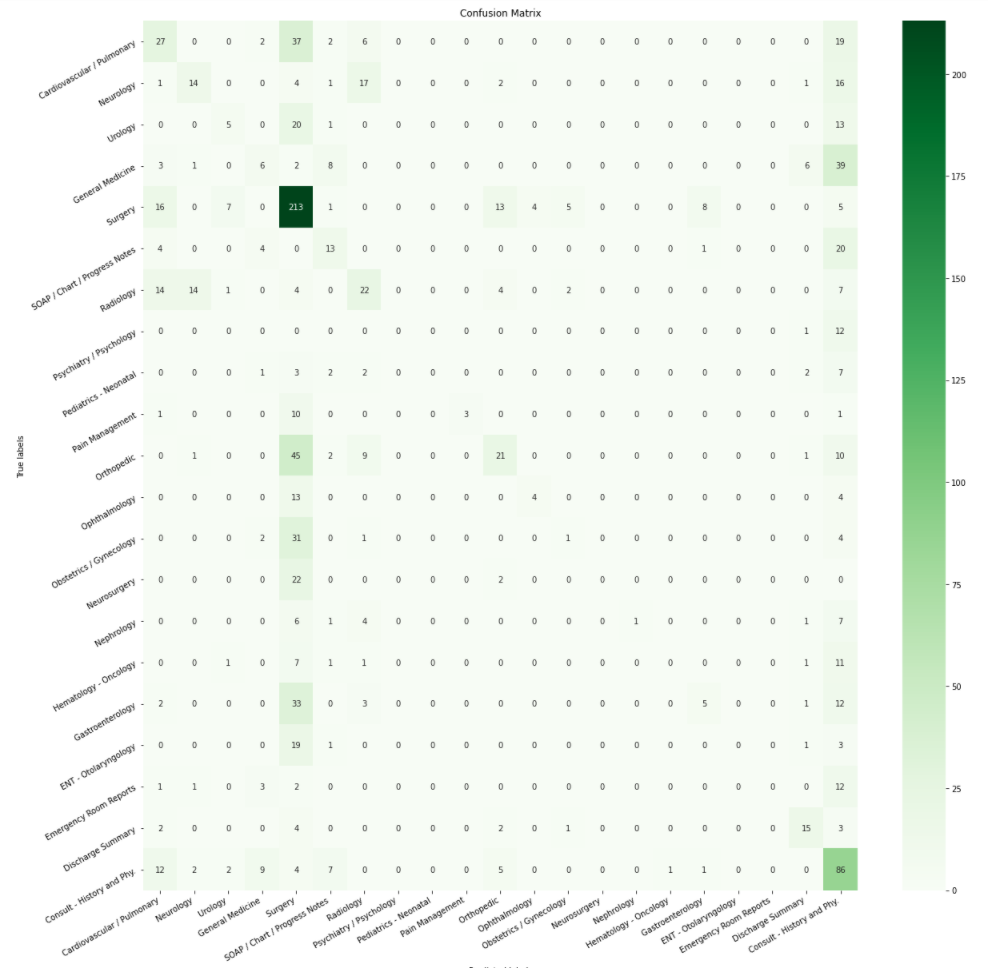
\includegraphics[width=\textwidth,height=20cm,keepaspectratio]{pictures/5.3cMatrix.png} 
\caption{Η γραφική απεικόνιση του πίνακα σύγχυσης}\label{figure5.3}
\end{figure}
\clearpage

H βιβλιοθήκη \en{sklearn} προσφέρει τη μέθοδο \en{classification\_report()} η οποία τυπώνει τις εκτιμήσεις διαφόρων μετρικών πάνω στην ποιότητα  των αποτελεσμάτων πρόβλεψεις του αλγορίθμου. 

Οι μετρικές αυτές είναι:
\begin{enumerate}
    \item Ορθότητα (\en{Accuracy)}
    \item Ανάκληση (\en{Recall)} 
    \item Ακρίβεια (\en{Precision)} 
    \item \en{F-Measure} 
\end{enumerate}

Τα πρώτα αποτελέσματα ακρίβειας ταξινόμησης ανά κατηγορία φαίνονται στον παρακάτω πίνακα (Σχήμα ~\ref{figure5.4}:
 
\begin{figure} [ht!]
\centering
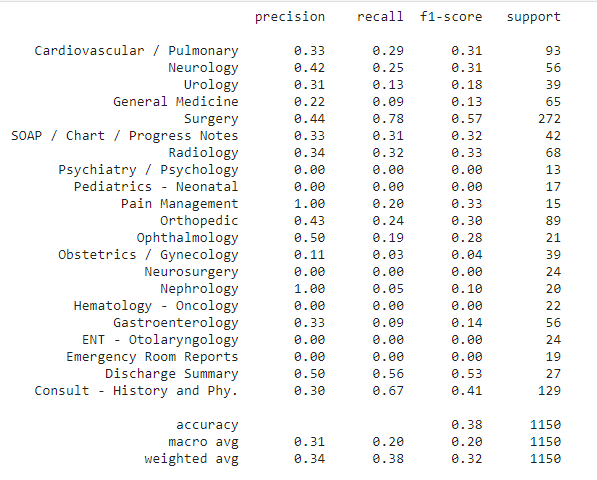
\includegraphics[width=\textwidth,height=20cm,keepaspectratio]{pictures/5.4results.png} 
\caption{Πίνακας πρώτων αποτελεσμάτων μετρικών ταξινόμησης}\label{figure5.4}
\end{figure}
\clearpage

Από το \en{classification report} παρατηρούμε ότι τα αποτελέσματα ακρίβειας είναι αρκετά χαμηλά. Αυτό οφείλεται στο οτι πολλές απο τις κατηγορίες αλληλοεπικαλύπτονται, όπως φαίνεται και στον πίνακα σύγχυσης. Επειδή αυτό συμβαίνει λόγω της φύσης των δεδομένων, καθώς σε κάποια περιστατικά δε γίνεται να αποφανθεί οτι εμπίπτουν μόνο σε μια συγκεκριμένη ιατρική ειδικότητα, στο επόμενο βήμα αφαιρούνται απο το σύνολο των δεδομένων οι ειδικότητες που δημιουργούν αυτόν το «θόρυβο».

Οι ειδικότητες που απαλείφονται είναι: 
\begin{enumerate}
    \en{\item Surgery
        \item SOAP / Chart / Progress Notes
        \item Consult - History and Phy.
        \item Emergency Room Reports
        \item Discharge Summary
        \item Pain Management
        \item General Medicine}
\end{enumerate}


Επίσης, λόγω κοινού γνωστικού πεδίου, συγχωνεύονται οι εξής κατηγορίες:
\begin{enumerate}
    \en{\item Neurosurgery \& Neurology
        \item Nephrology \& Urology}
\end{enumerate}

Ο πίνακας του πλήθους εγγραφών ανα κατηγορία μετά τη διαμόρφωση του έχει τη μορφή που παρουσιάζεται στο Σχήμα ~\ref{figure5.5}:
\begin{figure} [ht!]
\centering
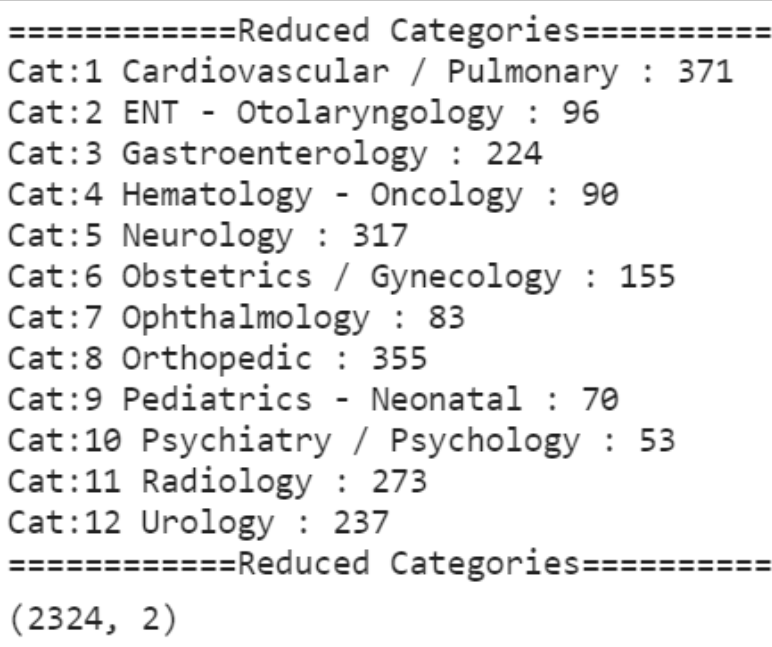
\includegraphics[width=\textwidth,height=7cm,keepaspectratio]{pictures/5.4reducedCat(12cat).png} 
\caption{Το πλήθος εγγραφών ανά κατηγορία μετά την απαλοιφή και τη συγχώνευση κάποιων κατηγοριών}\label{figure5.5}
\end{figure}


Το \en{sciSpacy} είναι ένα πακέτο της  \en{Python} το οποίο περιέχει τα μοντέλα  \en{Spacy} και είναι σχεδιασμένο για προεπεξεργασία σε κείμενα που περιέχουν οντότητες που αποτελούν ιατρική, επιστημονική ή κλινική ορολογία.

Αξιοποιώντας τη δυνατότητα αυτού του πακέτου, δημιουργείται η συνάρτηση \en{process\_text()} η οποία περνάει κάθε εγγραφή του πεδίου \en{transcription} ως είσοδο στη μέθοδο \en{nlp()} του μοντέλου \en{en\_ner\_bionlp13cg\_md} του πακέτου \en{sciSpacy}, η οποία επιστρέφει το σύνολο λέξεων που έχουν ιατρική, επιστημονική ή κλινική νοηματική αξία.


Έπειτα, εφαρμόζουμε αναδρομικά όλη τη διαδικασία:
\begin{enumerate}
    \item Προεπεξεργασία (εφαρμογή \en{sciSpacy})
    \item \en{Tf-Idf} αξιολόγηση
    \item Απεικόνιση του πίνακα \en{Tf-Idf} με χρήση της μεθόδου \en{t-SNE}
    \item Εφαρμογή \en{PCA} στον πίνακα \en{Tf-Idf}
    \item Εκ νέου διαχωρισμός δεδομένων σε \en{training set} και \en{test set}
    \item Εφαρμογή λογιστικής παλινδρόμησης \en{(logistic regression)}
    \item Κατασκευή Πίνακα Σύγχυσης \en{(confusion matrix)}
    \item Εμφάνιση νέων αποτελεσμάτων μετρικών ποιότητας πρόβλεψης
\end{enumerate}

Το Σχήμα~ \ref{figure5.6} εμφανίζει την απεικόνιση του πίνακα που προέκυψε από την \en{tf-idf} με χρήση της μεθόδου \en{t-SNE} μετά την εκ νέου προεπεξεργασία των δεδομένων 

\begin{figure} [ht!]
\centering
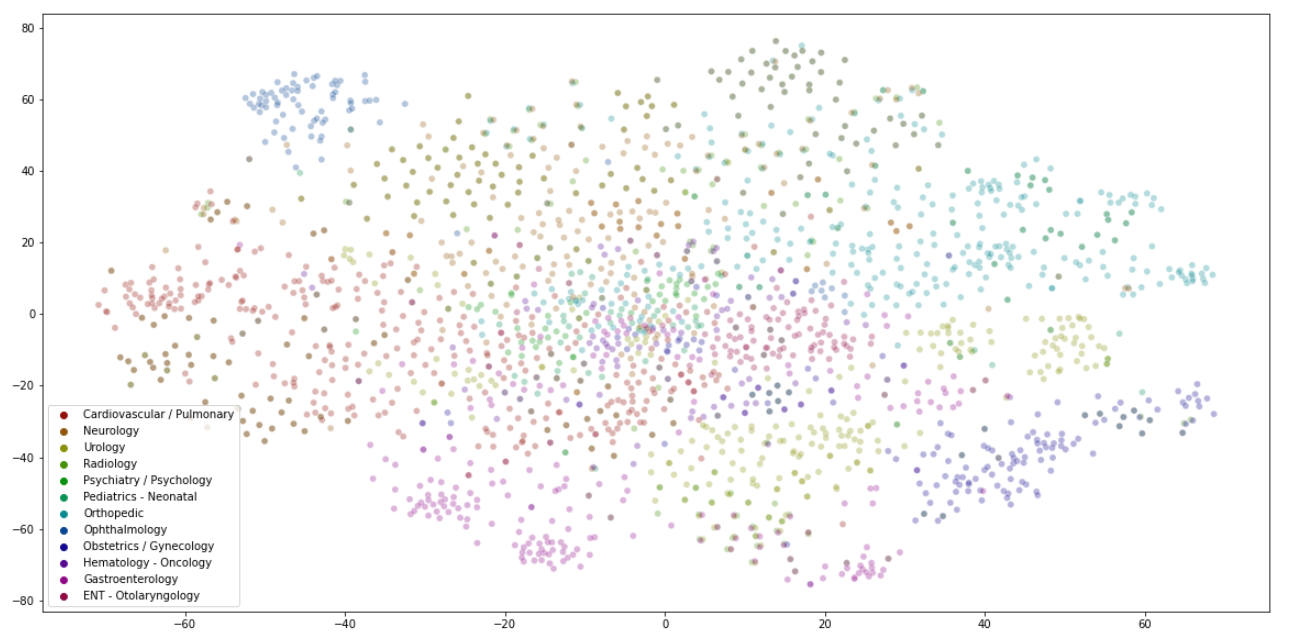
\includegraphics[width=\textwidth,height=12cm,keepaspectratio]{pictures/5.6tsne2.png} 
\caption{Η νέα γραφική απεικόνιση του αλγορίθμου \en{t-SNE}}\label{figure5.6}
\end{figure}


Ο νέος Πίνακας Σύγχυσης και ο νέος Πίνακας αποτελεσμάτων μετρικών ταξινόμησης φαίνονται στα σχήματα ~\ref{figure5.7} και ~\ref{figure5.8}

\begin{figure} [ht!]
\centering
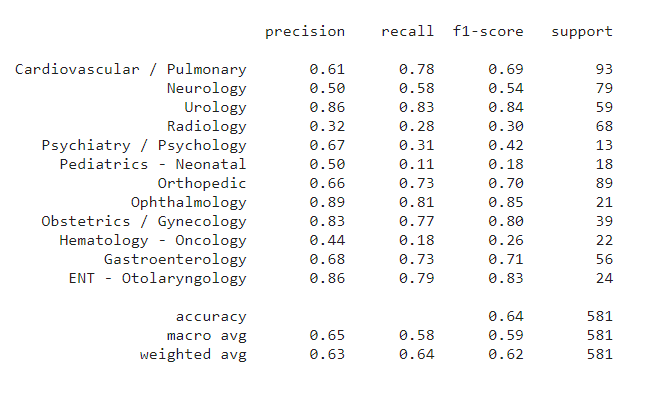
\includegraphics[width=\textwidth,height=8cm,keepaspectratio]{pictures/5.8results2.png} 
\caption{Πίνακας Αποτελεσμάτων μετρικών ταξινόμησης μετά την επεξεργασία με το πακέτο \en{sciSpacy}}\label{figure5.8}
\end{figure}

\begin{figure} [ht!]
\centering
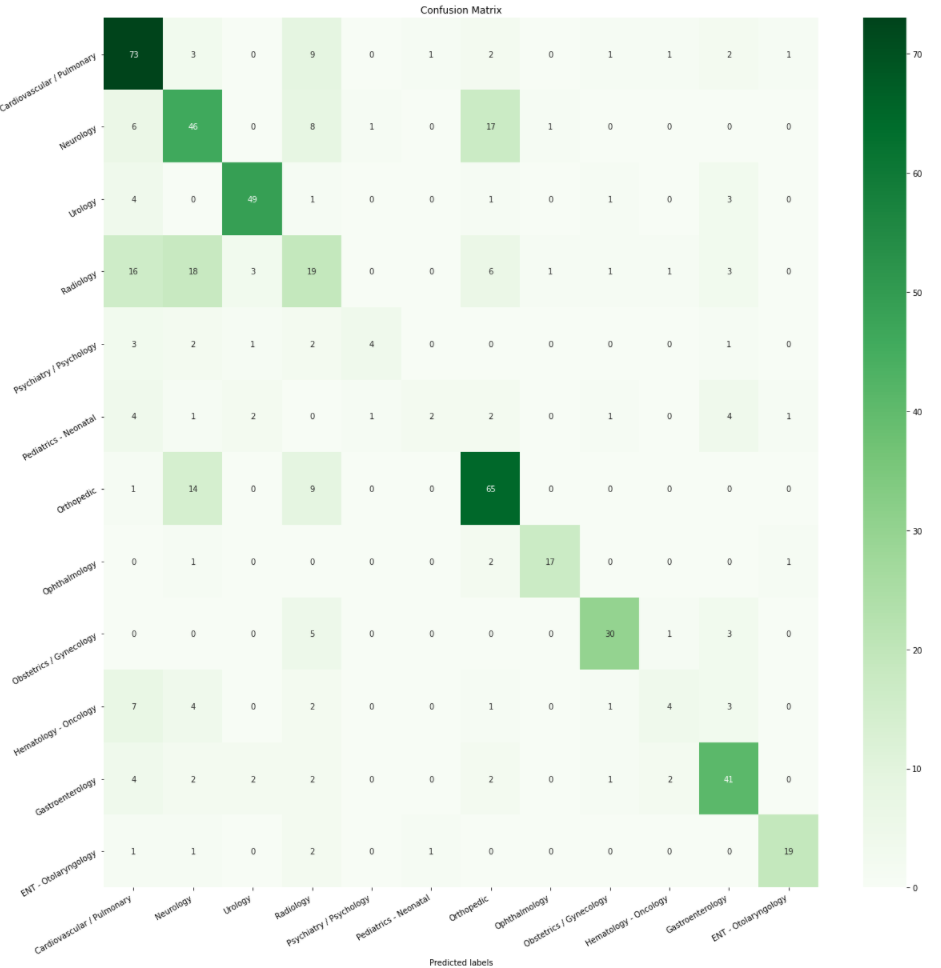
\includegraphics[width=\textwidth,height=12cm,keepaspectratio]{pictures/5.7cMatrix2.png} 
\caption{Πίνακας Σύγχυσης  μετά την επεξεργασία με το πακέτο \en{sciSpacy}}\label{figure5.7}
\end{figure}
\clearpage

Παρατηρούμε εμφανώς βελτιωμένα αποτελέσματα στα \en{scores} των διάφορων μετρικών. (προηγούμενα αποτελέσματα στο σχήμα ~\ref{figure5.4})
Παρ’ όλα αυτά, εξακολουθεί να υπάρχει ανισορροπία στο πλήθος των υπαρχόντων δεδομένων μεταξύ των κατηγοριών. 

Στα πλαίσια της συγκεκριμένης εργασίας ακολουθήθηκαν σε προηγούμενα βήματα και οι δύο προσεγγίσεις αντιμετώπισης της ανισορροπίας των δεδομένων \en{(oversampling} και \en{undersampling}: αφαιρέθηκαν οι κλάσεις που αποτελούσαν μειονότητες καθώς και η κλάση της χειρουρικής που περιείχε δεδομένα κατά πολύ μεγαλύτερα σε όγκο σε σχέση με τις υπόλοιπες κλάσεις τα οποία επίσης συγχέονταν με αυτές λόγω επικαλυπτόμενων γνωστικών πεδίων.

Μία ακόμα απλή προσέγγιση για την αντιμετώπιση του προβλήματος θα ήταν να χρησιμοποιηθεί η απλούστερη \en{oversampling} τεχνική η οποία υποδεικνύει τη δημιουργία διπλότυπων στιγμιοτύπων στις κατηγορίες που αποτελούν μειονότητες. Κάτι τέτοιο όμως, παρ' ότι φαινομενικά επιφέρει μεγαλύτερη ισορροπία στα δεδομένα, δεν προσθέτει καμία καινούρια πληροφορία στο μοντέλο εκπαίδευσης.

Γι' αυτό θα χρησιμοποιηθεί η τεχνική \en{SMOTE (Synthetic Minority Oversampling Technique)}.


Πριν τη δημιουργία νέου \en{dataset} με την τεχνική \en{SMOTE} τα δεδομένα ήταν τα εξής:
\en{
\begin{itemize}
    \item Train\_Set\_Size: (1743, 696)
    \item Test\_Set\_Size: (581, 696) 
\end{itemize}}


Μετά τη δημιουργία νέου \en{dataset} με την τεχνική \en{SMOTE} τα δεδομένα είναι τα εξής:
\en{
\begin{itemize}
    \item Train\_Set\_Size: (1981, 696)
    \item Test\_Set\_Size: (661, 696) 
\end{itemize}
}

\clearpage 
\subsection{Λογιστική Παλινδρόμηση }

Στη συνέχεια γίνεται εφαρμογή Λογιστικής Παλινδρόμησης και παράγεται ο νέος Πίνακας Σύγχυσης (Σχήμα ~ \ref{figure5.10}):

\begin{figure} [ht!]
\centering
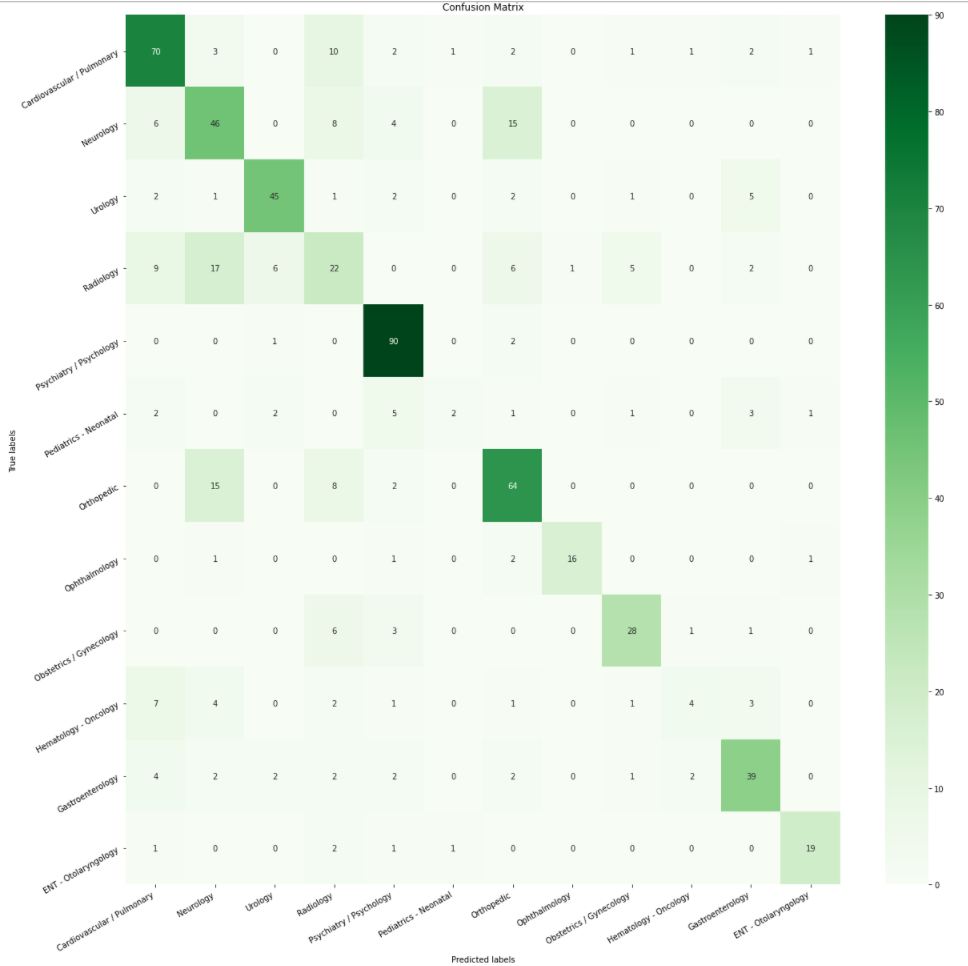
\includegraphics[width=\textwidth,height=12cm,keepaspectratio]{pictures/5.10CMatrix3.png} 
\caption{Πίνακας Σύγχυσης μετά την εφαρμογή της τεχνικής \en{SMOTE}}\label{figure5.10}
\end{figure}

\clearpage
Τέλος, δημιουργείται ο πίνακας των τελικών αποτελεσμάτων μετρικών ταξινόμησης ο οποίος φαίνεται στο σχήμα ~\ref{figure5.11}.

\begin{figure} [ht!]
\centering
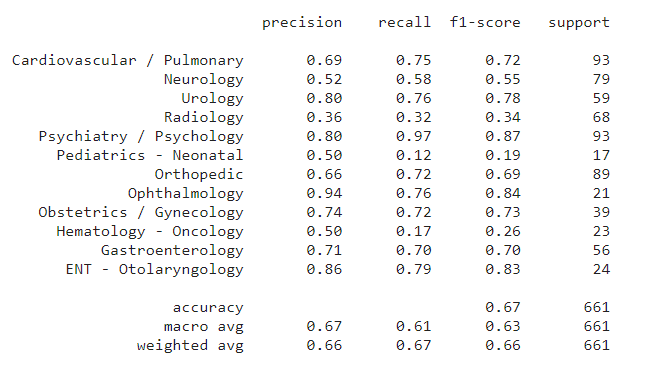
\includegraphics[width=\textwidth,height=8cm,keepaspectratio]{pictures/5.11results3.png} 
\caption{\en{Logistic Regression: }Πίνακας τελικών Αποτελεσμάτων μετρικών ταξινόμησης μετά την εφαρμογή της τεχνικής \en{SMOTE}}\label{figure5.11}
\end{figure}

Τα τελικά αποτελέσματα είναι εμφανώς βελτιωμένα. 
Παρατηρούμε οτι σε συγκεκριμένες κατηγορίες όπως \en{Neurology, Radiology} και \en{Hematology} τα αποτελέσματα ταξινόμησης παραμένουν χαμηλά καθώς οι περιγραφές των περιστατικών εξακολουθούν να αφορούν παραπάνω απο μία ειδικότητες. 


Στη συνέχεια, για την ταξινόμηση του κειμένου, δοκιμάζεται η επίδοση των αλγορίθμων:
\begin{enumerate}
    \item \en{Naïve Bayes} 
    \item \en{SVM}
    \item \en{kNN}
\end{enumerate}


διατηρώντας ως είσοδο το \en{dataset} στην τελευταία μορφή που ταξινομήθηκε με τη μέθοδο της λογιστικής παλινδρόμησης, πριν την επεξεργασία για επίτευξη \en{oversampling} με την τεχνική \en{SMOTE}.

\clearpage
\subsection{Αλγόριθμος \en{Naïve Bayes}}
Ο πίνακας αποτελεσμάτων των μετρικών ταξινόμησης που παράγεται από τη μέθοδο \en{classification\_report()} για τον Αλγόριθμο \en{Naïve Bayes} φαίνεται στο σχήμα ~\ref{figure5.12}.

\begin{figure} [ht!]
\centering
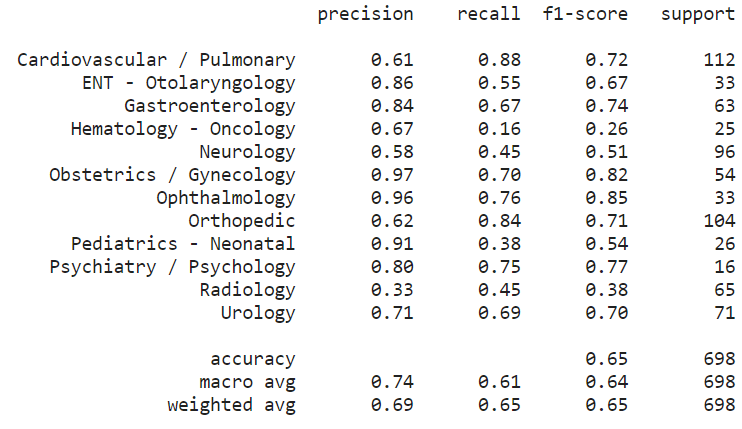
\includegraphics[width=\textwidth,height=8cm,keepaspectratio]{pictures/NAiveBAyes_NO_SMOTE.png} 
\caption{\en{Naïve Bayes: }Πίνακας Αποτελεσμάτων μετρικών ταξινόμησης}\label{figure5.12}
\end{figure}
\clearpage

\subsection{Αλγόριθμος \en{SVM}}

Ο πίνακας αποτελεσμάτων των μετρικών ταξινόμησης που παράγεται από τη μέθοδο \en{classification\_report()} για τον Αλγόριθμο \en{SVM} φαίνεται στο σχήμα ~\ref{figure5.13}.

\begin{figure} [ht!]
\centering
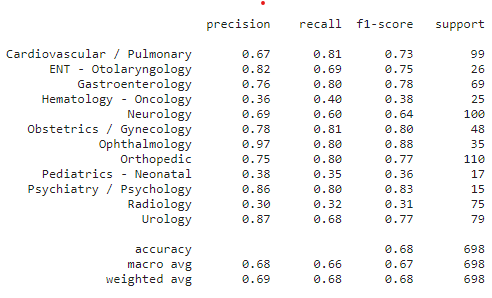
\includegraphics[width=\textwidth,height=8cm,keepaspectratio]{pictures/SVM_NO_SMOTE.png} 
\caption{\en{SVM: }Πίνακας Αποτελεσμάτων μετρικών ταξινόμησης}\label{figure5.13}
\end{figure}
\clearpage

\subsection{Αλγόριθμος \en{kNN}}
Ο πίνακας αποτελεσμάτων των μετρικών ταξινόμησης που παράγεται από τη μέθοδο \en{classification\_report()} για τον Αλγόριθμο \en{kNN} φαίνεται στο σχήμα ~\ref{figure5.14}.

\begin{figure} [ht!]
\centering
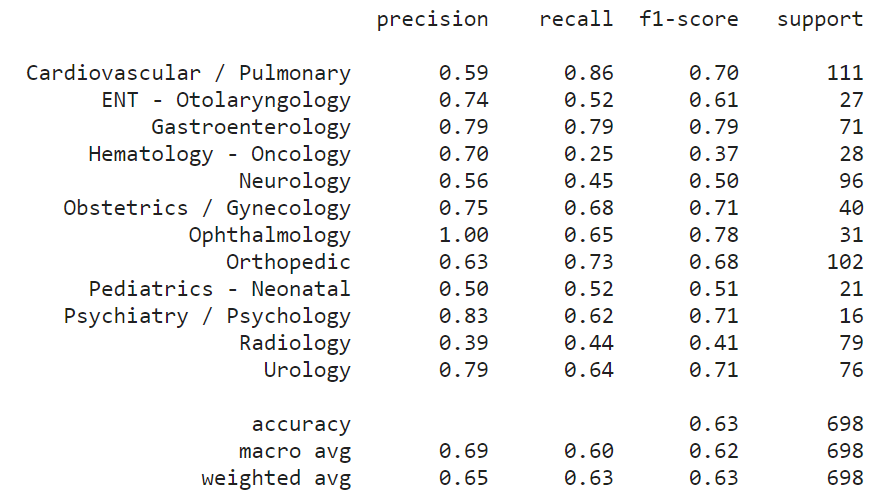
\includegraphics[width=\textwidth,height=8cm,keepaspectratio]{pictures/knn_NO_SMOTE.png} 
\caption{\en{kNN: }Πίνακας Αποτελεσμάτων μετρικών ταξινόμησης}\label{figure5.14}
\end{figure}




\subsection{\en{ΛΕΙΠΕΙ -> Word2Vec - Neural Network}}

\en{\subsubsection{Word Embedding}
Ο όρος Word Embedding είναι ο συλλογικός όρος για τεχνικές μάθησης χαρακτηριστικών όπου οι λέξεις από το λεξιλόγιο αντιστοιχίζονται σε διανύσματα πραγματικών αριθμών. Αυτά τα διανύσματα υπολογίζονται από την πιθανοτική κατανομή για κάθε λέξη που εμφανίζεται πριν ή μετά από μια άλλη. Με άλλα λόγια, λέξεις που εκφράζουν παρόμοιες έννοιες συνήθως εμφανίζονται μαζί στο σώμα κειμένου, επομένως θα είναι κοντά και στον χώρο των διανυσμάτων. 

Στα πλαίσια της παρούσας διπλωματικής, χρησιμοποιείται το πρώτο μοντέλο αυτής της οικογένειας: το Word2Vec της Google (2013). Άλλα δημοφιλή μοντέλα ενσωμάτωσης λέξης είναι το GloVe του Stanford (2014) και το FastText του Facebook (2016).

Το Word2Vec παράγει έναν χώρο διανυσμάτων, συνήθως με εκατοντάδες διαστάσεις, για κάθε διακριτή λέξη του κειμένου, έτσι ώστε οι λέξεις που εκφράζουν παρόμοιες έννοιες να βρίσκονται κοντά η μία στην άλλη στο διανυσματικό χώρο. Αυτό μπορεί να γίνει με δύο διαφορετικές προσεγγίσεις: ξεκινώντας από μια μεμονωμένη λέξη για να προβλέψουμε το συμφραζόμενο της (Skip-gram) ή ξεκινώντας από το συμφραζόμενο για να προβλέψουμε μια λέξη (Continuous Bag-of-Words).

Αρχικά μετατρέπουμε το σύνολο του dataset σε λίστα που περιέχει λίστες (list of lists), κάθε μία εκ των οποίων περιέχει το σύνολο των διακριτών λέξεων του κειμένου μιας εγγραφής.

Κατά την εφαρμογή του Word2Vec, θα πρέπει να καθοριστούν:
\begin{itemize}
    \item Το επιθυμητό μέγεθος των διανυσματικών αναπαραστάσεων των λέξεων. Επιλέχθηκε η τιμή 300.
    \item Το παράθυρο (window), δηλαδή τη μέγιστη απόσταση μεταξύ της τρέχουσας και της προβλεπόμενης λέξης μέσα σε μια πρόταση. Στη συγκεκριμένη υλοποίηση επιλέχθηκε το μέσο μήκος του κειμένου στη συλλογή (TODO: ελεγχος)
    \item Tον αλγόριθμο εκπαίδευσης.  Επιλέχθη η μέθοδος skip-grams (sg=1), καθώς γενικά παρουσιάζει καλύτερα αποτελέσματα.
\end{itemize}

}